
%(BEGIN_QUESTION)
% Copyright 2013, Tony R. Kuphaldt, released under the Creative Commons Attribution License (v 1.0)
% This means you may do almost anything with this work of mine, so long as you give me proper credit

This P\&ID is for an {\it anaerobic digester}, which takes in cow manure and preconsumer food waste (e.g. waste products from slaughterhouses, fish processing plants, etc.) and generates flammable methane gas which is used as fuel for an engine generator, producing electricity and usable heat from agricultural waste.  

$$\includegraphics[width=15.5cm]{i0015rx01.eps}$$

Heat from the engine's circulating coolant is used to maintain the digester at around 100 $^{o}$F for optimum methane gas generation, because the mildly exothermic reaction of anaerobic methane production does not create enough heat to maintain its own temperature at optimum levels:

$$\hbox{C}_6\hbox{H}_{12}\hbox{O}_6 \to \hbox{CO}_2 + \hbox{CH}_4 \hskip 30pt \Delta H = -34.6 \hbox{ kcal/mol}$$

\vskip 10pt

Suppose you were asked to tune the zone temperature controllers (TIC-1, TIC-2, and TIC-3) in this process.  Answer the following questions regarding tuning:

\begin{itemize}
\item{} Which controller would you tune first, or does it matter?
\item{} Do you suspect these zones will be {\it self-regulating}, {\it integrating}, or {\it runaway} processes?
\item{} Should these controllers be tuned P-dominant or I-dominant?  Explain your reasoning.
\item{} What precautions, if any, would you need to take when tuning these controllers?  Are there any safety considerations we would need to be aware of before beginning the tuning procedure?
\item{} Identify any {\it loads} in the process, and explain how you would adjust them in order to test the robustness of your controller tuning.
\item{} Do you suppose the tuning parameters of TIC-1 will be much different from those used in TIC-3?  Explain why or why not.
\item{} What process change(s) would be required in order for the anaerobic reaction to be self-sustaining in terms of heat, so that an external heat source would not be required to sustain its operation at around 100 $^{o}$F?
\item{} Suppose maintenance personnel had to enter the digester vessel to physically clean the heat-exchange ``coils'' of fouling.  What personal safety precautions would they need to take before entering the vessel?
\end{itemize}

\underbar{file i04777}
%(END_QUESTION)





%(BEGIN_ANSWER)

\begin{itemize}
\item{} Which controller would you tune first, or does it matter? {\it You should definitely tune TIC-1 before TIC-2, and TIC-2 before TIC-3.  If you don't, then poor tuning in an upstream controller may present an unstable load to downstream controllers, thus complicating your tuning efforts.}
\vskip 10pt
\item{} Do you suspect these zones will be {\it self-regulating}, {\it integrating}, or {\it runaway} processes? {\it They should be self-regulating, with a long (slow) first-order time constant.}
\vskip 10pt
\item{} Should these controllers be tuned P-dominant or I-dominant?  Explain your reasoning.  {\it The tuning will most likely be P-dominant, as a purely first-order lag process should respond very well to aggressive controller action, and the large mass of liquid makes ``noise'' in the PV signal unlikely.}
\vskip 10pt
\item{} What precautions, if any, would you need to take when tuning these controllers?  Are there any safety considerations we would need to be aware of before beginning the tuning procedure? {\it This is a fairly safe process to tune.  No amount of temperature swing capable from engine coolant as the heat source will cause the slurry to become chemically or physically unstable.  At worse, you might risk killing off the bacterial culture if the process remains much too hot for much too long, but this would require a severe temperature excursion.}
\vskip 10pt
\item{} Identify any {\it loads} in the process, and explain how you would adjust them in order to test the robustness of your controller tuning. {\it Influent flow rate is definitely one load, adjustable by the setpoint on FIC-4.  Engine coolant temperature is another load, but this is harder to adjust since it is set by the engine's mechanical thermostat (these are normally non-adjustable).}
\vskip 10pt
\item{} Do you suppose the tuning parameters of TIC-1 will be much different from those used in TIC-3?  Explain why or why not. {\it Probably not, unless the zones differ substantially in volume.}
\vskip 10pt
\item{} What process change(s) would be required in order for the anaerobic reaction to be self-sustaining in terms of heat, so that an external heat source would not be required to sustain its operation at around 100 $^{o}$F? {\it Influent/effluent heat exchangers would be necessary to capture as much heat from the digested slurry as possible and put that heat into the incoming slurry, as well as lots of thermal insulation surrounding the digester vessel itself (to prevent heat loss).  The major problem here is the sheer mass of water in the slurry, water having a high specific heat capacity.  This requires a lot of heat energy in order to raise its temperature even by small amounts.  If the incoming feed is at ambient temperature, the amount of heat necessary to raise the slurry's temperature to 100 $^{o}$F will be likely much more than the amount of heat liberated by the digesting sugars, which means it will require ``help'' in the form of heat exchange with the hot effluent in order to achieve this temperature.  Furthermore, even if all these measures were in place, the start-up time of such a process would be very long without some external heat source to get it going.}
\vskip 10pt
\item{} Suppose maintenance personnel had to enter the digester vessel to physically clean the heat-exchange ``coils'' of fouling.  What personal safety precautions would they need to take before entering the vessel?  {\it As the digester vessel is most definitely a ``confined space,'' personnel would have to first flush it of all dangerous materials (including slurry), purge the space with fresh air, and check oxygen concentrations with a safety analyzer before entering.  Once inside, a person standing outside with a safety rope would have to stand watch in case anyone were to become incapacitated for some reason inside the vessel.}
\end{itemize}


%(END_ANSWER)





%(BEGIN_NOTES)


\filbreak \vskip 20pt \vbox{\hrule \hbox{\strut \vrule{} {\bf Virtual Troubleshooting} \vrule} \hrule}

\noindent
{\bf Predicting the effect of a given fault:} present each of the following faults to the students, one at a time, having them comment on all the effects each fault would produce.

\begin{itemize}
\item{} 
\item{} 
\item{} 
\end{itemize}


\vskip 10pt


\noindent
{\bf Identifying possible/impossible faults:} present symptoms to the students and then have them determine whether or not a series of suggested faults could account for all the symptoms, explaining {\it why} or {\it why not} for each proposed fault:

\begin{itemize}
\item{} Symptom: {\it }
\item{} 
\item{} 
\item{} 
\end{itemize}


\vskip 10pt


\noindent
{\bf Determining the utility of given diagnostic tests:} present symptoms to the students and then propose the following diagnostic tests one by one.  Students rate the value of each test, determining whether or not it would give useful information (i.e. tell us something we don't already know).  Students determine what different results for each test would indicate about the fault, if anything:

\begin{itemize}
\item{} Symptom: {\it }
\item{}  -- {\bf Yes/No}
\item{}  -- {\bf Yes/No}
\end{itemize}


\vskip 10pt


\noindent
{\bf Diagnosing a fault based on given symptoms:} imagine the ??? fails ??? in this system (don't reveal the fault to students!).  Present the operator's observation(s) to the students, have them consider possible faults and diagnostic strategies, and then tell them the results of tests they propose based on the following symptoms, until they have properly identified the nature and location of the fault:

\begin{itemize}
\item{} {\it }
\item{} 
\item{} 
\end{itemize}

%INDEX% Basics, control loop troubleshooting (realistic P&ID shown)
%INDEX% Process: anaerobic digester 

%(END_NOTES)


